\section{Sharp truncation of the log-gamma moment expansion}
Use the constants $\tau,\rho,C$ of the preceding late-coefficient theorem,
and put $\Lambda=-\log\rho$. In this section write $b_k=c_k>0$ for those
positive coefficients, and $\widetilde c_k=(-1)^{k-1}b_k$. The real inverse
$g(t)$ of $1/\Gamma(x)$ on $0\le x\le1$ satisfies $g(t)=-h(-t)$, where
$h(w)=w\Gamma(1-h(w))$ is the earlier inverse germ. Thus
$g(t)=\sum_{k\ge1}\widetilde c_k t^k$ near zero. The moment integral is
\[
 m_n:=M_n/n!=\frac1{\Gamma(n)}\int_0^\infty y^{n-1}g(e^{-y})\,dy.
\]
The first relative coefficient $d_1$ below is the earlier $\beta_1$.
Set $P=\psi'(-\tau)$, $Q=\psi''(-\tau)$, and $R=\psi^{(3)}(-\tau)$; equivalently
$d_1=R/(8P^2)-5Q^2/(24P^3)$.

\begin{lemma}[The dominant inverse singularity]\label{sharp:lem:slit}
The germ $g$ continues to a slit disk of radius greater than $\rho$,
with its only singularity on $|t|=\rho$ at $t=-\rho$, a square-root branch point.
\end{lemma}
\begin{proof}
The positive inverse $h$ has $h(\rho)=\tau$ and is absolutely convergent on
that circle. Its positive coefficients of degrees one and two imply
$|h(t)|<\tau$ at every other point of the circle. With
$\Phi(u)=\Gamma(1-u)$, one then has
$|t\Phi'(h(t))|\le\rho\Phi'(|h(t)|)<\rho\Phi'(\tau)=1$.
The implicit-function theorem continues the inverse across those points.
At $t=\rho$, local inversion at the simple critical point gives a convergent
square-root expansion. Compactness supplies a slightly larger slit disk;
replace $t$ by $-t$ for $g$. This verifies the usual smooth implicit-function
hypotheses directly.\cite{sharp:FS}
\end{proof}
\subsection{A uniform Taylor-remainder lemma}

The next statement is the key passage from fixed-order asymptotics to
optimal truncation. It explicitly crosses the radius of convergence on
the positive real axis; merely summing an infinite Taylor tail there
would be invalid.

\begin{lemma}[Uniform inverse remainder]\label{sharp:lem:inverse-remainder}
For some \(\delta>0\), uniformly for
\(t\in[\rho e^{-\delta},\rho e^\delta]\), put \(r=t/\rho\). Then
\begin{equation}\label{sharp:eq:inverse-remainder}
 \frac{g(t)-\sum_{k=1}^{N-1}\widetilde c_kt^k}{\widetilde c_Nt^N}
 =\frac1{1+r}+\frac{3r}{2N(1+r)^2}+O(N^{-2}).
\end{equation}
On each of the remaining real intervals
\(0<t\leq\rho e^{-\delta}\) and
\(\rho e^\delta\leq t\leq1\), the same normalized remainder is
bounded uniformly in \(N\) sufficiently large.
\end{lemma}

\begin{proof}
The preceding theorem gives a slit disk of continuation for \(g\),
with its only singularity at \(-\rho\).
Choose its outer radius \(R>\rho\), and then \(\delta>0\) so small that
\(\rho e^\delta<R\) and \(\rho e^\delta<1\).
Cauchy's integral formula for \(g(t)\), less its first \(N-1\)
Taylor terms, has kernel \(t^N/(z^N(z-t))\). Deform its contour to the
two banks of the negative cut and an outer contour.
The coefficient \(\widetilde c_N\) uses kernel \(z^{-N-1}\).
On the cut \(z=-s\), the ratio of these kernels, after removing
\(t^N\), is
\[
 \frac{z}{z-t}=\frac{s}{s+t}.
\]
The jump of \(g\) at \(s=\rho\) is a nonzero constant times
\((s-\rho)^{1/2}(1+O(s-\rho))\), with a complete expansion.
The coefficient integral is thus a Watson-type endpoint integral
whose normalized variable \(u=(s-\rho)/\rho\) has
\[
 \langle u\rangle=\frac{3}{2N}+O(N^{-2}),
 \qquad \langle u^2\rangle=O(N^{-2}).
\]
These formulas follow directly by comparing
\(\int_0^\epsilon u^{j+1/2}(1+u)^{-N-1}\dd u\)
with its beta integral extended to infinity. Terms outside a fixed
small neighborhood of zero are exponentially smaller.
Expanding
\[
 \frac{s}{s+t}
 =\frac1{1+r}+\frac{r}{(1+r)^2}u+O(u^2)
\]
proves \eqref{sharp:eq:inverse-remainder}.
The outer contour contributes \(O(R^{-N})\) to the coefficient and
\(O((t/R)^N)\) to the remainder; after normalization these errors are
exponentially small uniformly on the stated compact \(t\)-interval.
This contour argument defines and estimates the actual analytic
remainder on both sides of \(t=\rho\).

It remains to bound the two outer real intervals.
The estimate \(b_k\asymp\rho^{-k}k^{-3/2}\) implies that, below
\(\rho e^{-\delta}\), the absolutely convergent tail is bounded by
a constant times \(b_Nt^N\). Above \(\rho e^\delta\), use
\[
 \sum_{k<N}\frac{b_kt^k}{b_Nt^N}
 \ll\sum_{k<N}(N/k)^{3/2}(\rho/t)^{N-k}.
\]
Splitting at \(k=N/2\) bounds this uniformly by a geometric series
plus an exponentially small term times a polynomial in \(N\).
Furthermore \(0\leq g(t)\leq1\), whereas \(b_Nt^N\) grows
exponentially uniformly on this interval. This proves the last claim.
\end{proof}

\subsection{Sharp optimal truncation}

\begin{theorem}[Half the first omitted term]\label{sharp:thm:optimal-moment}
Let \(n,N\) tend to infinity through positive integers with
\(\eta=N\Lambda-n\) in a fixed bounded interval. Then
\begin{equation}\label{sharp:eq:optimal-moment}
 \boxed{\displaystyle
 m_n-\sum_{k=1}^{N-1}\frac{(-1)^{k-1}b_k}{k^n}
 =\frac{(-1)^{N-1}b_N}{N^n}
 \left(\frac12+\frac{3-2\eta}{8N}+O(N^{-2})\right).}
\end{equation}
The \(O\)-constant is uniform for bounded \(\eta\).
The ratio in parentheses has a complete asymptotic expansion in
\(1/N\), with coefficients computable from the local inverse expansion
and gamma moments.
In particular, taking the nearest integer to \((n+3/2)/\Lambda\)
gives a rigorously justified least-term approximation. The error
eventually has the sign of the first omitted term and is asymptotic
to one half of that term.
\end{theorem}

\begin{proof}
Subtract the finite sum under \eqref{gaussian:eq:moment-inverse}, using
\[
 \frac1{(n-1)!}\int_0^\infty y^{n-1}e^{-ky}\dd y=k^{-n}.
\]
With \(Y\) having the gamma density
\(N^ny^{n-1}e^{-Ny}/(n-1)!\), the error divided by \(\widetilde c_N/N^n\) is
the expectation of the normalized inverse remainder at \(t=e^{-Y}\).

The gamma distribution concentrates at \(\Lambda\):
\[
 \E Y=\frac nN=\Lambda-\frac\eta N,\qquad
 \operatorname{Var}Y=\frac n{N^2}.
\]
For every fixed small \(\delta>0\), its probability outside
\([\Lambda-\delta,\Lambda+\delta]\) is \(O(e^{-a_\delta N})\).
This follows from its moment-generating function
\((1-u/N)^{-n}\) and Chernoff's inequality.
The uniform outer bounds in Lemma~\ref{sharp:lem:inverse-remainder}
therefore make the outer contribution exponentially small.

On the middle interval, the leading kernel is
\[
 L(Y-\Lambda)=\frac1{1+e^{\Lambda-Y}},\qquad
 L(v)=\frac12+\frac v4-\frac{v^3}{48}+O(v^4).
\]
Writing \(V=Y-\Lambda\), its centered gamma moments give
\[
 \E V=-\frac\eta N,\qquad
 \E V^3=O(N^{-2}),\qquad \E V^4=O(N^{-2}),
\]
uniformly for bounded \(\eta\). Thus
\(\E L(V)=1/2-\eta/(4N)+O(N^{-2})\).
It is essential here to use the signed third moment; an absolute
cubic bound alone would lose half a power.
The correction kernel in \eqref{sharp:eq:inverse-remainder} is
\[
 \frac{3e^{-V}}{2N(1+e^{-V})^2}.
\]
Its value at zero is \(3/(8N)\), and its first derivative vanishes
there, so its expectation is \(3/(8N)+O(N^{-2})\).
Adding these terms proves \eqref{sharp:eq:optimal-moment}.
The contour calculation and the Taylor/gamma-moment calculation can
both be continued to arbitrary fixed order. Gamma central moments
are polynomials in \(n\) and \(N^{-1}\); their parity and degree give
integer powers of \(N^{-1}\).
\end{proof}

The theorem strengthens the classical expansion in two ways.
It allows \(N\) to grow linearly with \(n\), and it estimates the
actual error after truncation. The least-term estimate alone would
not justify either conclusion. No global sign assertion for every
\(n,N\) is needed.

\begin{corollary}[Second correction]\label{sharp:cor:moment-second}
Under the hypotheses of Theorem~\ref{sharp:thm:optimal-moment}, the normalized
error has the more precise expansion
\begin{align}
 \frac{m_n-\sum_{k<N}\widetilde c_k/k^n}{\widetilde c_N/N^n}
 &=\frac12+\frac{3-2\eta}{8N}\notag\\
 &\quad+\frac1{N^2}
 \left(\frac{d_1}{4}+\frac{\Lambda(6\eta-13)}{96}\right)
 +O(N^{-3}).\label{sharp:eq:moment-second}
\end{align}
\end{corollary}

\begin{proof}
Here are the additional local coefficients, so that the assertion is
independently reproducible. Let \(v=B-\tau\), and use \(P,Q,R\)
from \eqref{sharp:lem:slit}. The characteristic inverse satisfies
\[
 \log\frac{B/\Gamma(1-B)}{\rho}
 =-\frac{P}{2}v^2+\frac{Q}{6}v^3-\frac{R}{24}v^4+O(v^5).
\]
Putting \(w=\sqrt{1-t/\rho}\) and
\(\alpha_*=\sqrt{2/P}\), inversion gives
\[
 B(t)=\tau-\alpha_* w+\frac{Q}{3P^2}w^2+\mu w^3+O(w^4),
 \qquad
 D:=\frac{\mu}{\alpha_*}
 =-\frac14+\frac{R}{12P^2}-\frac{5Q^2}{36P^3}.
\]
Thus the positive cut density for \(B\) is
\((\alpha_*/\pi)u^{1/2}(1+Du+O(u^2))\), where \(u=t/\rho-1\).
Transfer gives \(d_1=3/8+3D/2\), proving
\eqref{sharp:lem:slit} as well. The normalized endpoint moments are
\[
 \langle u\rangle=\frac{3}{2N}
       +\frac{9/4+3D/2}{N^2}+O(N^{-3}),\qquad
 \langle u^2\rangle=\frac{15}{4N^2}+O(N^{-3}),\qquad
 \langle u^3\rangle=O(N^{-3}).
\]
They follow from beta integrals and the displayed cut density.
The coefficient of \(N^{-2}\) in the inverse remainder at \(r=t/\rho\)
is therefore
\[
 K_2(r)=\frac{r}{(1+r)^2}\left(\frac94+\frac{3D}{2}\right)
                    -\frac{15r}{4(1+r)^3},\qquad K_2(1)=d_1/4.
\]
For the gamma average, put
\(K_1(v)=3e^{-v}/[2(1+e^{-v})^2]\) and \(V=Y-\Lambda\).
Taylor expansion through degree five, using
\(\E|V|^6=O(N^{-3})\), gives
\[
 \E L(V)=\frac12-\frac{\eta}{4N}
       +\frac{\Lambda(3\eta-2)}{48N^2}+O(N^{-3}),\qquad
 \E K_1(V)=\frac38-\frac{3\Lambda}{32N}+O(N^{-2}).
\]
For example \(\E V^3=\Lambda(2-3\eta)N^{-2}+O(N^{-3})\);
the signed fifth moment is \(O(N^{-3})\).
Also \(\E K_2(e^{-V})=K_2(1)+O(N^{-1})\).
The uniform outer bound again makes all outer contributions
exponentially small. Combining the three terms proves
\eqref{sharp:eq:moment-second}.
\end{proof}

\begin{figure}[t]
 \centering
 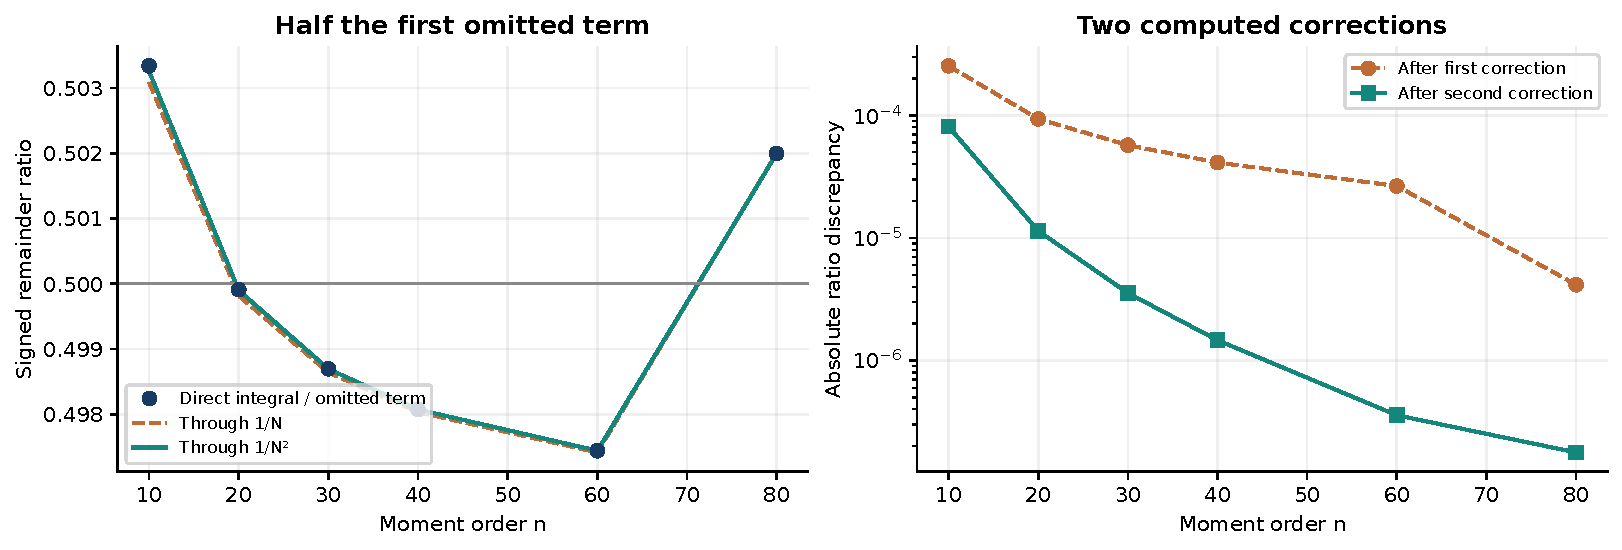
\includegraphics[width=\textwidth]{../reports/reflection-euler-tornheim/figures/moment_remainders.pdf}
 \caption{The signed error divided by the first omitted term, at a
 truncation near \((n+3/2)/\Lambda\). The first-correction formula tracks
 the small changes caused by rounding the truncation index. The plot is
 numerical corroboration; Theorem~\ref{sharp:thm:optimal-moment} supplies the proof.}
 \label{sharp:fig:moments}
\end{figure}

\subsection{A convergent identity with an explicit tail bound}

An asymptotic series should not be used as an infinite exact sum.
The same inverse coordinate gives an exact convergent alternative.

\begin{proposition}[Cutoff identity]\label{sharp:prop:cutoff}
For \(n\geq1\) and \(Y>\Lambda\),
\begin{equation}\label{sharp:eq:cutoff}
 m_n=\frac1{(n-1)!}\int_0^Y y^{n-1}g(e^{-y})\dd y
      +\sum_{k\geq1}\frac{\widetilde c_k}{k^n}Q(n,kY),
 \qquad
 Q(n,z)=e^{-z}\sum_{j=0}^{n-1}\frac{z^j}{j!}.
\end{equation}
The sum is absolutely convergent. If \(Y>\log4\), the absolute tail
after \(k=K\) is at most
\begin{equation}\label{sharp:eq:cutoff-bound}
 \frac{(4e^{-Y})^{K+1}}{2(1-4e^{-Y})}
 \sum_{j=0}^{n-1}\frac{Y^j}{j!(K+1)^{n-j}}.
\end{equation}
\end{proposition}

\begin{proof}
Split \eqref{gaussian:eq:moment-inverse} at \(Y\), substitute the convergent inverse
series on the tail, and integrate term by term.
The coefficient growth theorem proves absolute convergence.
For the elementary explicit bound, note that
\[
 \frac{1/2}{\Phi(1/2)}=\frac1{2\sqrt\pi}>\frac14.
\]
The smaller solution to \(B=t\Phi(B)\) at \(t=1/4\) is therefore
less than \(1/2\); equivalently \(B(1/4)<1/2\).
Positivity gives \(b_k\leq4^k/2\).
For \(k>K\) and \(j\leq n-1\), \(k^{j-n}\leq(K+1)^{j-n}\).
The geometric tail now gives \eqref{sharp:eq:cutoff-bound}.
\end{proof}

The numerical implementation uses ordinary high-precision arithmetic
and explicitly distinguishes analytic truncation bounds from interval
rounding bounds. Formula \eqref{sharp:eq:cutoff} is also suitable for a future
ball-arithmetic evaluator: the finite inverse integral and all constant
evaluations can be enclosed separately.

